\documentclass[tikz,border=12pt]{standalone}
\usepackage[T1]{fontenc}
\usepackage[utf8]{inputenc}
\usepackage{lmodern}
\usetikzlibrary{arrows.meta}

% Evolução coordenada DSQ--RSQ: versão VERTICAL (colunas em vez de faixas).
% Esquerda->direita: azul (DSQ) | amarelo (RSQ) | vermelho (desdobramento).
% Tempo corre de cima para baixo em cada coluna (t0 no topo, tn embaixo).
\definecolor{ink}{HTML}{25344A}
\definecolor{muted}{HTML}{617287}
\definecolor{blueband}{HTML}{E8F2FA}
\definecolor{blueborder}{HTML}{3B78AA}
\definecolor{yellowband}{HTML}{FFF3D7}
\definecolor{yellowborder}{HTML}{C98A28}
\definecolor{redband}{HTML}{F9E9EA}
\definecolor{redbox}{HTML}{AF343B}

\tikzset{
  stage/.style={
    rectangle, rounded corners=4pt, draw=ink!55, fill=white,
    line width=0.8pt, text width=2.42cm, minimum height=1.15cm,
    align=center, inner xsep=5pt, inner ysep=5pt,
    font=\small
  },
  digital/.style={stage, draw=blueborder!80},
  real/.style={stage, draw=yellowborder!85},
  evolution digital/.style={-{Latex[length=2.5mm]}, draw=blueborder,
    line width=1.15pt, line cap=round},
  evolution real/.style={-{Latex[length=2.5mm]}, draw=yellowborder,
    line width=1.15pt, line cap=round},
  guidance/.style={-{Latex[length=2.4mm]}, draw=muted,
    line width=0.9pt, dashed},
  outcome link/.style={-{Latex[length=2.4mm]}, draw=redbox!80,
    line width=1pt, line cap=round}
}

\begin{document}
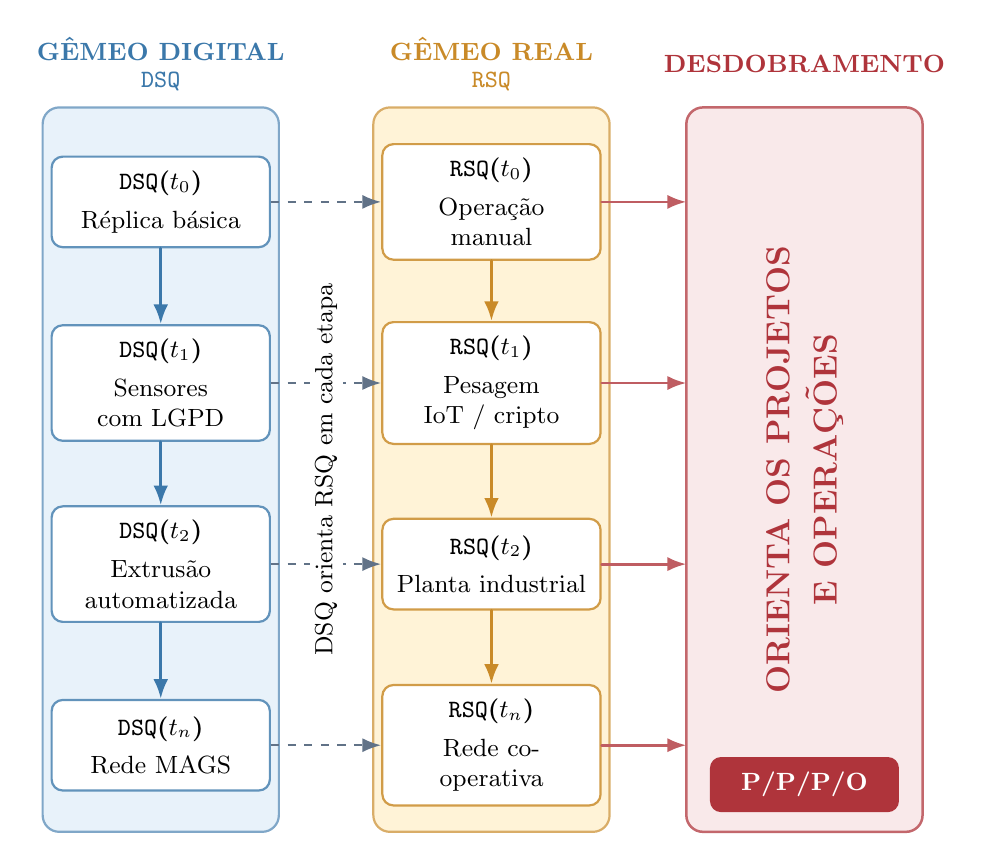
\begin{tikzpicture}[font=\sffamily]

  % ---- Colunas de fundo: azul (esquerda) / amarelo (meio) / vermelho
  % (direita). Mesma lógica de cores e espessuras das faixas originais,
  % só que giradas 90°: espessura da coluna = largura do nó (2.42cm) +
  % respiro, altura da coluna = span dos 4 instantes de tempo.
  % Vãos entre colunas reduzidos em 25%: azul->amarelo 1.6->1.2,
  % amarelo->vermelho 1.3->0.975. Largura/altura das colunas intactas.
  \filldraw[fill=blueband, draw=blueborder!65, line width=0.8pt,
            rounded corners=6pt]
    (-1.5,1.4) rectangle (1.5,10.6);
  \filldraw[fill=yellowband, draw=yellowborder!70, line width=0.8pt,
            rounded corners=6pt]
    (2.7,1.4) rectangle (5.7,10.6);
  \filldraw[fill=redband, draw=redbox!75, line width=0.9pt,
            rounded corners=6pt]
    (6.675,1.4) rectangle (9.675,10.6);

  % Rótulos de coluna, acima de cada faixa (equivalente aos rótulos de
  % trilha da versão horizontal, que ficavam à esquerda de cada linha).
  \node[align=center, text=blueborder, font=\bfseries\small]
    at (0,11.15) {GÊMEO DIGITAL\\[-1pt] \normalfont\texttt{DSQ}};
  \node[align=center, text=yellowborder, font=\bfseries\small]
    at (4.2,11.15) {GÊMEO REAL\\[-1pt] \normalfont\texttt{RSQ}};
  \node[align=center, text=redbox, font=\bfseries\small]
    at (8.175,11.15) {DESDOBRAMENTO};

  % ---- Estados alinhados por tempo: agora descendo, não mais da
  % esquerda para a direita. t0 no topo, tn embaixo.
  \node[digital] (d0) at (0,9.4)
    {{\bfseries\texttt{DSQ}($t_0$)}\\[3pt] Réplica básica};
  \node[digital] (d1) at (0,7.1)
    {{\bfseries\texttt{DSQ}($t_1$)}\\[3pt] Sensores com LGPD};
  \node[digital] (d2) at (0,4.8)
    {{\bfseries\texttt{DSQ}($t_2$)}\\[3pt] Extrusão automatizada};
  \node[digital] (dn) at (0,2.5)
    {{\bfseries\texttt{DSQ}($t_n$)}\\[3pt] Rede MAGS};

  \node[real] (r0) at (4.2,9.4)
    {{\bfseries\texttt{RSQ}($t_0$)}\\[3pt] Operação manual};
  \node[real] (r1) at (4.2,7.1)
    {{\bfseries\texttt{RSQ}($t_1$)}\\[3pt] Pesagem IoT / cripto};
  \node[real] (r2) at (4.2,4.8)
    {{\bfseries\texttt{RSQ}($t_2$)}\\[3pt] Planta industrial};
  \node[real] (rn) at (4.2,2.5)
    {{\bfseries\texttt{RSQ}($t_n$)}\\[3pt] Rede cooperativa};

  % Setas verticais = avanço temporal em cada trilha (era horizontal).
  \draw[evolution digital] (d0.south) -- (d1.north);
  \draw[evolution digital] (d1.south) -- (d2.north);
  \draw[evolution digital] (d2.south) -- (dn.north);
  \draw[evolution real] (r0.south) -- (r1.north);
  \draw[evolution real] (r1.south) -- (r2.north);
  \draw[evolution real] (r2.south) -- (rn.north);

  % Setas horizontais tracejadas = orientação DSQ -> RSQ em cada etapa
  % (era vertical). Rótulo gira 90° para caber no vão estreito entre
  % as colunas azul e amarela.
  \draw[guidance] (d0.east) -- (r0.west);
  \draw[guidance] (d1.east) -- (r1.west);
  \draw[guidance] (d2.east) -- (r2.west);
  \draw[guidance] (dn.east) -- (rn.west);
  % Letra 25% maior (7pt -> 8.75pt) e preta, para ficar mais legível.
  \node[rotate=90, fill=white, inner xsep=5pt, inner ysep=2pt,
        text=black, font=\fontsize{8.75}{10.5}\selectfont]
    at (2.1,6.0) {DSQ orienta RSQ em cada etapa};

  % ---- Coluna de desdobramento: links saem de cada estado RSQ para a
  % borda esquerda da coluna vermelha (era a borda superior da faixa).
  % Agora toda a coluna (tag + texto) gira 90°, igual ao rótulo acima.
  \foreach \r/\y in {r0/9.4, r1/7.1, r2/4.8, rn/2.5}
    \draw[outcome link] (\r.east) -- (6.675,\y);

  \node[rotate=0, fill=redbox, text=white, rounded corners=4pt,
        minimum width=2.40cm, minimum height=0.70cm,
        font=\bfseries\small] at (8.175,2) {P/P/P/O};
  % Quebra manual (não depende do auto-wrap do text width): força
  % exatamente 2 linhas, sem cortar palavra no meio.
  \node[rotate=90, text=redbox, align=center, font=\bfseries\large,
        text width=7cm]
    at (8.175,6) {ORIENTA OS PROJETOS \\[3pt] E OPERAÇÕES};

\end{tikzpicture}
\end{document}